% Ch5.tex

\chapter{Estimating frog calling activity and species richness based on acoustic event detection and multi-label learning}
\label{cha:cha7ML}


\section{Overview}
\label{sect:introduction}

This chapter describes the research conducted for estimating frog calling activity and species richness. Different from Chapter \ref{cha:cha6MIML} that use AED for estimating frog species richness, AED is used to estimate the frog calling activity in this chapter.
In Chapter \ref{cha:cha6MIML}, acoustic features are calculated based on the results of AED to estimate frog species richness, but the accuracy of AED results directly affect the MIML classification performance.
To reduce the bias introduced by AED, this research presents global feature representations for the classification of recordings with multiple frog species. The feature representation is extracted from the whole recording without the syllable segmentation. Therefore, the classification process can be framed as a ML learning task.  



Three global feature representations are calculated to classify each 10-second recording: LPCs, MFCCs, and PWSCCs. Both MFCCs and PWSCCs are similar to the features used in Chapter \ref{cha:cha5WaveletFeature}. The difference is that each 10-second recording is divided into three equal parts, and both MFCCs and PWSCCs are calculated from each part and combined as the final feature, which can obtain more temporal information.


Furthermore, this proposed classification framework is conducted for a long-term analysis. Both frog calling activity and species richness during the breeding season are estimated. Also, the correlations between frog calling activity/species richness with weather variables are studied to reflect the relationship between them. 

  
The architecture of this frog calling activity and species richness estimation system is shown in Figure \ref{fig:Ch7_flowchart}. The system contains three parts: frog calling activity estimation, frog species richness estimation, and correlation analysis. Each part is discussed in detail in the following subsections.

\begin{figure}[htb!]
\centering
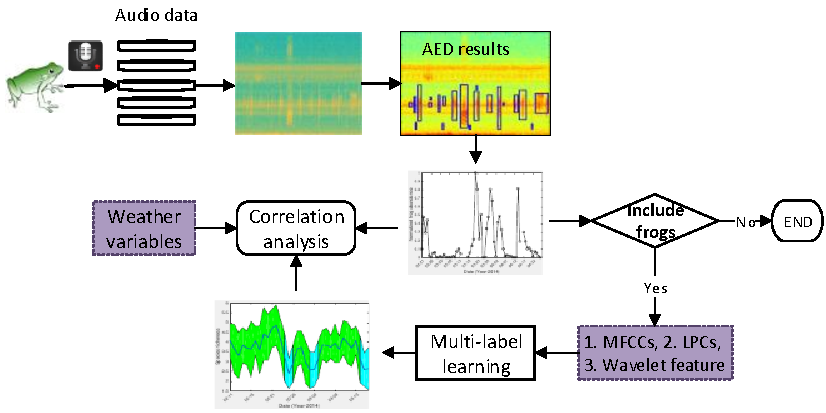
\includegraphics[width=\textwidth]{image/Ch7/flowchart.pdf}
\caption{Flowchart of a frog call classification system using AED and ML learning}
\label{fig:Ch7_flowchart}
\end{figure}


\section{Acquisition of frog call recordings}

To evaluate the proposed algorithm, the same dataset with Chapter~\ref{cha:cha6MIML} is used. The description of this dataset can be found in Chapter~\ref{chap5:Materials}. Besides the representative dataset, this study  sampled 10-second recordings every 10 minutes from continuous recordings over three months. Finally, there are 4170, 4908, and 1544 10-second recordings for \textit{Kiyomi dam}, \textit{Stony Creek dam} and \textit{BG Creek dam}, respectively, which are used for long-term acoustic monitoring. Here, the number of recordings of there sites is different due to the data loss in some days.




We first manually inspect spectrograms of ten randomly selected call examples for each frog species. Two parameters, dominant frequency and syllable duration, are measured and averaged, as listed in Table \ref{tab:Ch7_parameters}, which are used as prior information for subsequent analysis.



\section{Experiment setup}
Each 10-second recording is divided into frames of 512 samples and 50\% frame overlap for STFT. $A_{large}$ and $A_{small}$, which are used for area filtering in AED, are empirically set at 3000 pixels and 300 pixels, respectively. Allowed fluctuations in both sides of dominant frequency are 300 Hz for dominant frequency filtering. For WP-based feature, window size and overlap are 512 samples and 50\%, the window function is a Hamming window. All algorithms were programmed in Matlab 2014b except ML learning, which was implemented in Meka 1.7.7\footnote[4]{http://meka.sourceforge.net/}. 




\section{Frog calling activity}

\subsection{Frog calling activity of each 10-second recording}
Frog calling activity is estimated through the detection of acoustic events in a spectrogram image. Here, the spectrogram is generated by applying short-time Fourier transform (STFT) to each 10-second recording. The description of the AED method is shown in Chapter \ref{Ch5:AEDmethod}.



The frog calling activity of each 10-second recording is estimated as 

\begin{equation}
F_{abun} = \sum_{n=1}^{N}\sum_{i=1}^{I}\sum_{j=1}^{J} A_{i,j}(n)^2
\end{equation}
Here, $A_{i,j}$ represents the decibel value of location $(i,j)$ within each acoustic event $n$ in the spectrogram, $i$ is the temporal index, $j$ is the frequency index, $I$ and $J$ are the height and width of each acoustic event.

\begin{figure}
        \centering       
        \begin{subfigure}[b]{0.35\textwidth}
                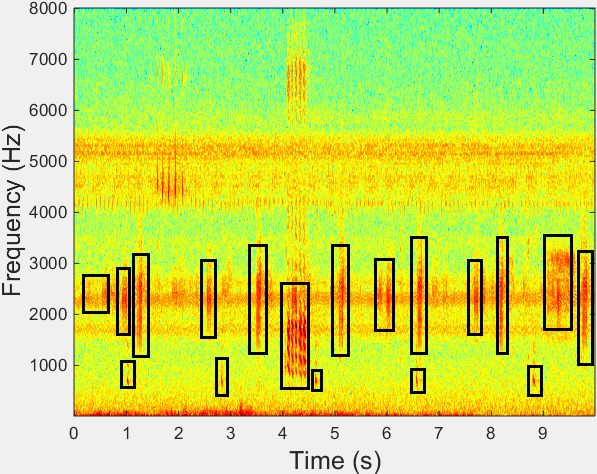
\includegraphics[width=\textwidth]{image/Ch7/spectrogram1-m.png}
                \caption{Baseline}
        \end{subfigure}%
 ~       
        \begin{subfigure}[b]{0.35\textwidth}
                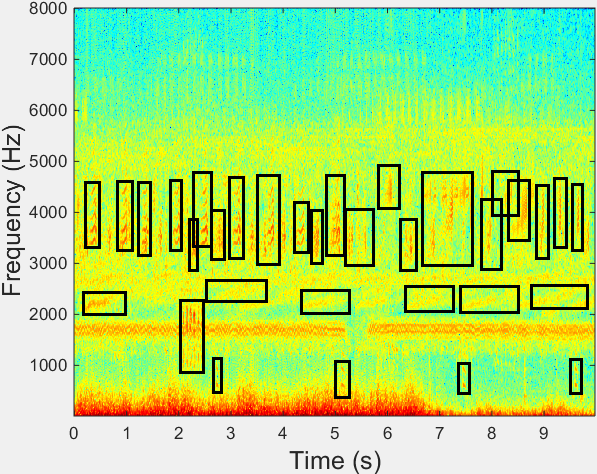
\includegraphics[width=\textwidth]{image/Ch7/spectrogram2-m.png}
                \caption{Baseline}
        \end{subfigure}%
        \\          
        \begin{subfigure}[b]{0.35\textwidth}
                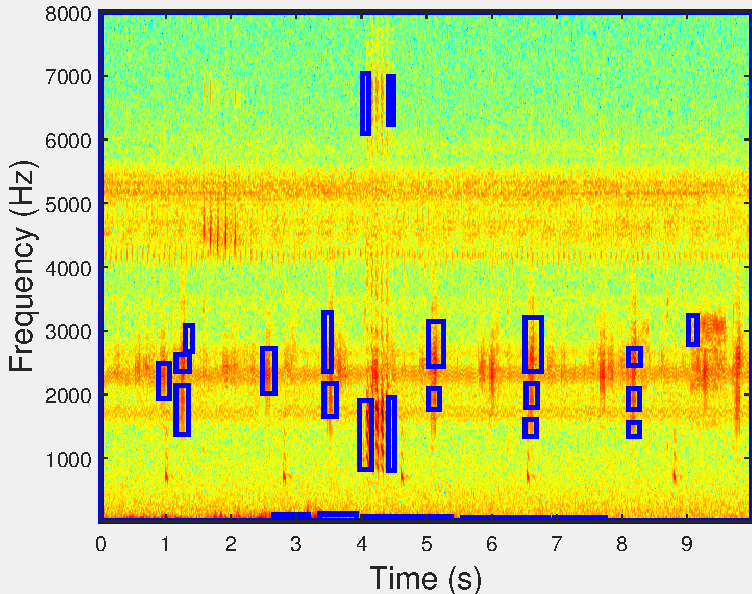
\includegraphics[width=\textwidth]{image/Ch7/AEDFodor.pdf}
                \caption{Method of \cite{fodor2013ninth}}
        \end{subfigure}%
                ~        
        \begin{subfigure}[b]{0.35\textwidth}
                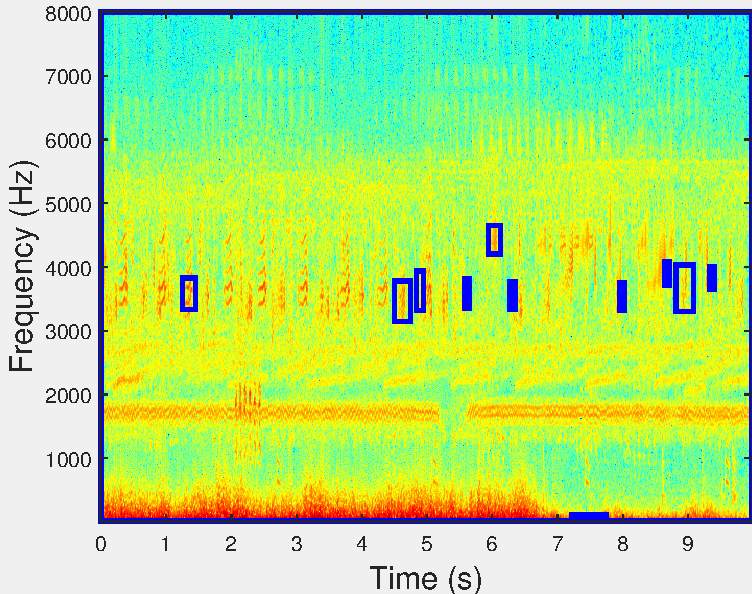
\includegraphics[width=\textwidth]{image/Ch7/AEDFodor_2.pdf}
                \caption{Method of \cite{fodor2013ninth}}
        \end{subfigure}
\\

               \begin{subfigure}[b]{0.35\textwidth}
                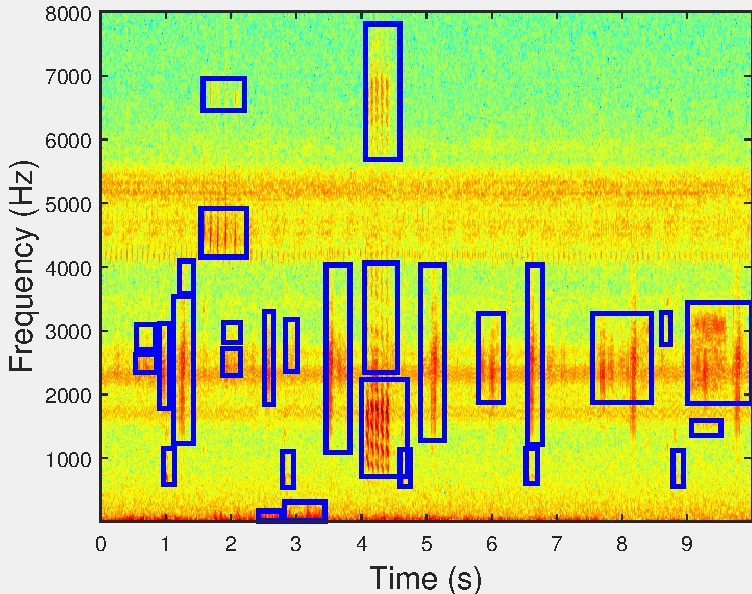
\includegraphics[width=\textwidth]{image/Ch7/AED_Michael.pdf}
                \caption{Method of \cite{Michael2011}}
        \end{subfigure}  
        ~  
                \begin{subfigure}[b]{0.35\textwidth}
                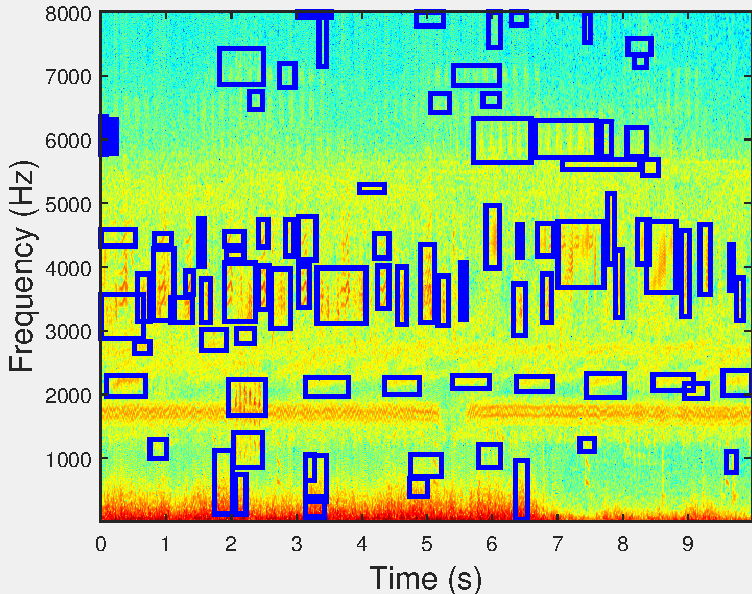
\includegraphics[width=\textwidth]{image/Ch7/AED_Michael_2.pdf}
                \caption{Method of \cite{Michael2011}}
        \end{subfigure}%              
\\         
                \begin{subfigure}[b]{0.35\textwidth}
       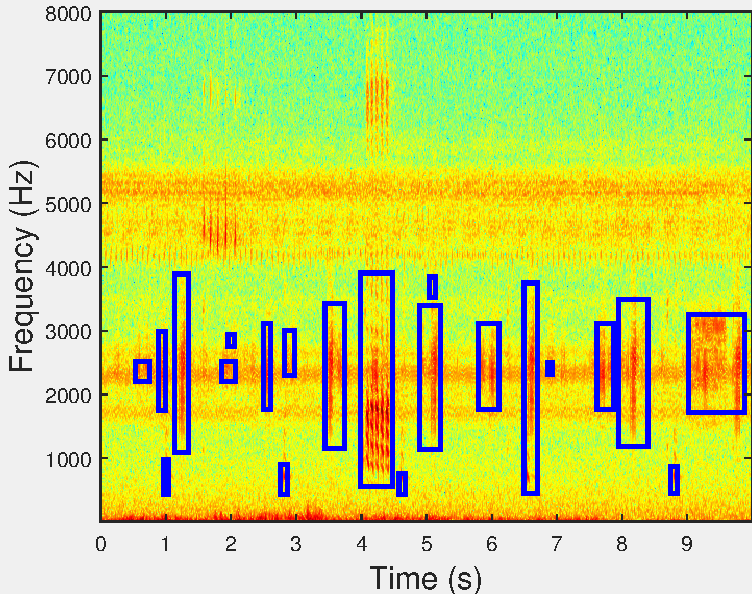
\includegraphics[width=\textwidth]{image/Ch7/AED_Jie.pdf}
                \caption{Proposed method}
        \end{subfigure}     
~
        \begin{subfigure}[b]{0.35\textwidth}
       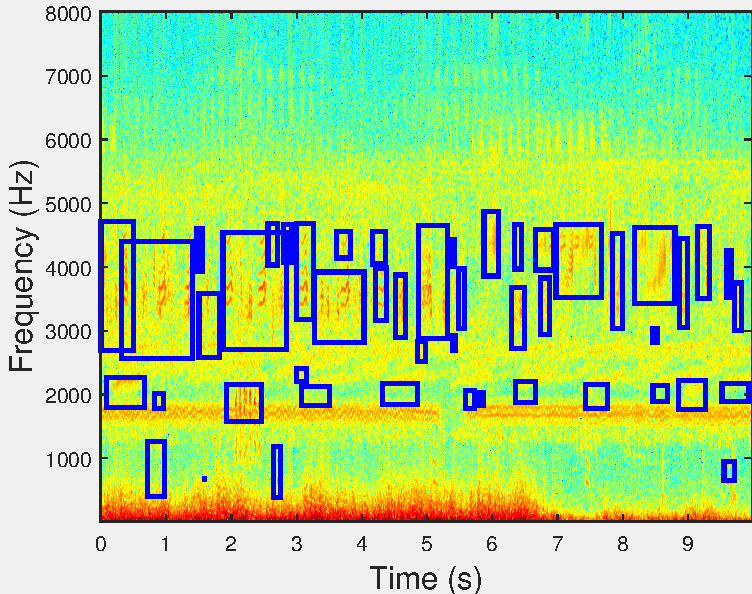
\includegraphics[width=\textwidth]{image/Ch7/AED_Jie_2.pdf}
                \caption{Proposed method}
        \end{subfigure}                
        \caption[AED for frog abundance monitoring using different methods]{AED for frog calling activity estimation using different methods. For each row, different methods are applied to the same recordings. The baseline of the detection results is shown in the first row; detected frog calls are drawn using a blue rectangle. For each column, different methods are used for the same recording.}        
        \label{fig:Ch7_AED}
\end{figure}


\subsection{Long-term monitoring of frog calling activity}

Figure~\ref{fig:frogAbundance} shows the frog calling activity results of three selected sites over the whole frog breeding season. It can be found that the frog calling activity of the same site changes a great deal over time. In the \textit{Kiyomi dam}, frog calling activity is relatively high from February 21 to February 25. However, frog calling activity is quite low in two periods, which are February 26 to March 11 and April 07 to April 12. The highest calling activity of this site is achieved on March 22. However, the highest calling activity for \textit{Stony Creek dam} and \textit{BG Creek dam} is obtained in February, which shows that frog calling activity of different sites often varies a lot for different environments. Recordings of 47 days of all three sites do not frog calls. In the subsequent analysis, only those recordings with frog calls are used for frog species richness estimation. 

\begin{figure}[htb!]
\centering
        \begin{subfigure}[b]{0.3\textwidth}
                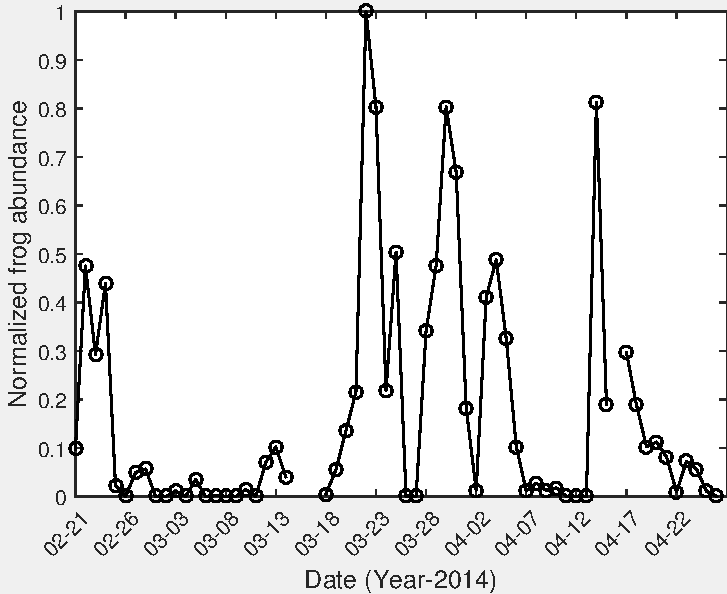
\includegraphics[width=\textwidth]{image/Ch7/abundance1075.pdf}
                \caption{\textit{Kiyomi dam}}
        \end{subfigure}
       ~
              \begin{subfigure}[b]{0.3\textwidth}
                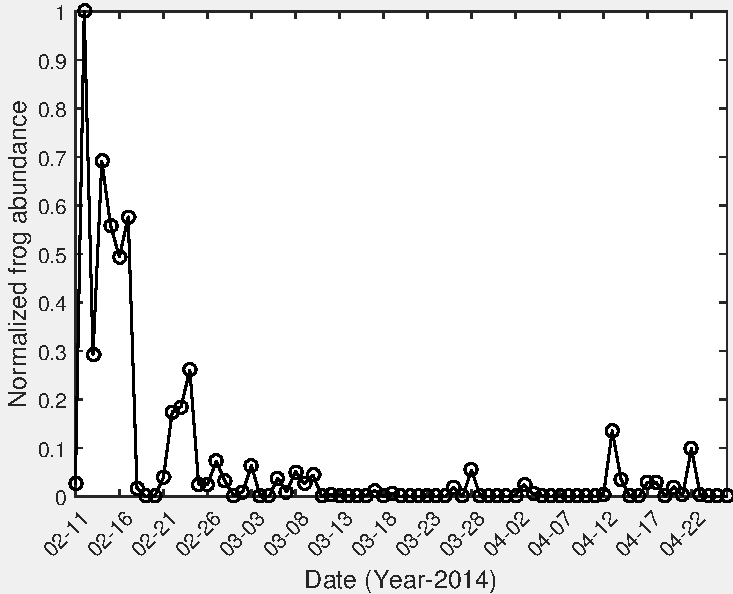
\includegraphics[width=\textwidth]{image/Ch7/abundance1078.pdf}     
                \caption{\textit{Stony creek dam}}           
        \end{subfigure} 
               ~
              \begin{subfigure}[b]{0.3\textwidth}
                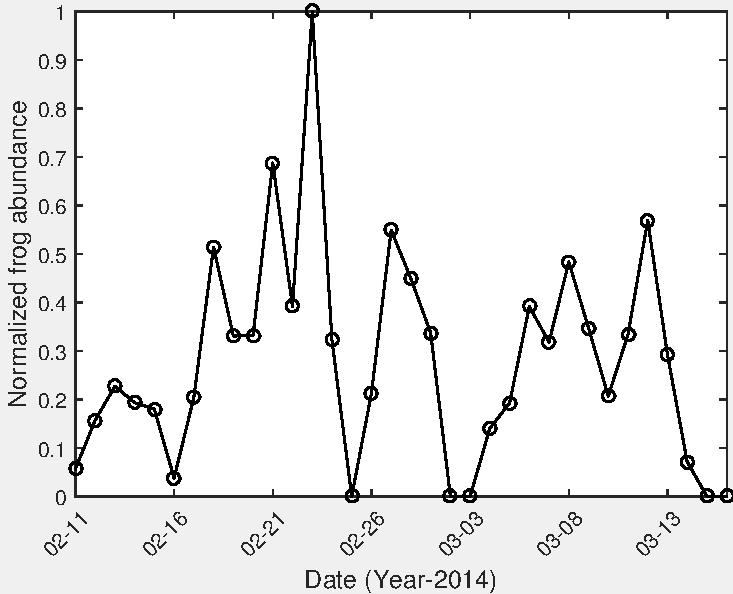
\includegraphics[width=\textwidth]{image/Ch7/abundance1079.pdf}     
                \caption{\textit{BG creek dam}}           
        \end{subfigure}       
\caption[Frog calling activity detection of different sites]{Frog calling activity estimation of different sites: \textit{Kiyomi dam}, \textit{Stony Creek dam} and \textit{BG Creek dam}. For \textit{Kiyomi dam}, three days do not record any acoustic data and then there is no value in those particular days. All the frog calling activity value is normalised to [0 1].}
        \label{fig:frogAbundance}
\end{figure}




\section{Frog species richness}


Frog species richness is estimated by predicting the species presence/absence of each sampled recording. Since many sampled recordings consist of multiple frog species, one direct solution is to assign each recording with a set of labels (frog species) for explicitly expressing its semantics \citep{ZhangReview2014}. Therefore, ML learning is adopted to classify each sampled recording. 

Extracting discriminating features, which maximise between-group (inter-specie) dissimilarity
and minimise within-group (intra-specie) dissimilarity, is very important for achieving high classification performance \citep{huang2009frog, bedoya2014automatic}. In this chapter, feature extraction is performed based on WPD using a modified version of the method introduced in Chapter \ref{cha:cha5WaveletFeature} and detailed below. 

For feature extraction, constructing a suitable frequency scale for a WP tree based on the dominant frequency of each frog species is the first step, because different frog species tend to have different dominant frequencies \citep{Gingras2013}. In Chapter \ref{cha:cha5WaveletFeature}, k-means clustering was first applied to the extracted dominant frequencies of training data. Then, the frequency scale was built by sorting clustering centroids to construct the WP tree. In this chapter, the prior information on dominant frequency  ($F_{0}$) obtained from Table \ref{tab:Ch7_parameters} is directly used to construct the WP tree. We iteratively detect each WP tree sub-band node until the frequency range of each node includes more than one dominant frequency $F_{0}$. Then, the WP tree of that particular sub-band node will be further split until each sub-band node has only one dominant frequency value or none. After constructing the frequency scale, adaptive frequency scaled WPD is applied to each sampled recording for feature extraction. The detailed description for extracting the features is shown in Chapter~\ref{Ch5:WPDfeature}.



The difference is that the recording is first split into frames using a Hamming window. Then, all frames are divided into three equal parts, and the WP-feature within each part is averaged, respectively, because different frog species within similar frequency bands may exist in one 10-second recording, splitting each recording into small parts might be able to keep the information of different frog species in the same frequency band. Besides the WP-based feature, two other acoustic features, LPCs and MFCCs, are calculated for the comparison.




\subsection{Multi-label classification for species richness estimation} 
Since many sampled recordings consist of calls from multiple frog species, frog call classification can be framed as a ML learning problem. However, previous studies have not adopted ML learning to classify frog calls. Therefore, it is worth investigating different ML learning algorithms for the classification of multiple vocalising frog species. In this chapter, four ML learning algorithms, whose base classifier is a C4.5 decision tree, are employed: binary relevance (BR), classifier chains (CC), random k-label sets (RAKEL and RAKEL1) \citep{ZhangReview2014}. The default parameter settings of those four ML learning algorithms are used. The trained classifier, which achieves the best classification performance, is then used to predict the presence/absence of the rest recordings. Lastly, frog species richness can be estimated as

\begin{equation}
F_{rich} = \frac{\sum_{k=1}^{K}f_{rich}(k)}{K}
\end{equation} 
where $f_{rich}(k)$ is the number of frog species of each 10-second recording with predicted labels, $K$ is the number of 10-second recording for each day.





\subsection{Frog species richness analysis}
Different ML learning algorithms are applied on 342 selected recordings to compare different feature sets. Then, five evaluation rules are used to compare the performance with the combination of four feature sets and four ML learning algorithms: hamming loss, rank loss, one error, example based F1, and micro F1 \citep{Madjarov20123084, ZhangReview2014}. The descriptions of hamming loss, rank loss, and one error can be found in Chapter~\ref{ch6:eveluationMetric}. The descriptions of example based F1  and micro F1 are shown as follows.



\textbf{(1)}
Example based $F_{1}$ is the average of the harmonic mean of instance-precision and instance-recall for every instance. The instance-precision is defined for an instance as the size of the intersection of the set of its predicted labels and the set of its ground truth labels divided by the size of the set of its predicted labels. The instance-recall is defined for an instance as the size of the intersection of the set of its predicted labels and the set of its ground truth labels divided by the size of the set of its ground truth labels.
\begin{equation}
macroF_{1}=\frac{1}{Q}\sum_{j=1}^{Q}\frac{2 \times p_{j} \times r_{j}}{p_{j}+r_{j}}
\end{equation}
where $p_{j}$ and $r_{j}$ are the precision and recall for all $\lambda_{h} \in h(x_{i})$ from $\lambda_{j} \in y_{j}$.
\\
\textbf{(2)}
Micro $F_{1}$ is the harmonic mean of micro-precision and micro-recall, where micro-precision and micro-recall are the precision and the recall which are averaged over all instances and label pairs. 
\begin{equation}
microF_{1} = \frac{2 \times microPrecision \times microRecall}{microPrecision + microRecall}
\end{equation}



Experiment results are shown in Table~\ref{tab:classificationResults}.

\begin{table}[htb!]
\centering
\caption[Classification results based on four feature sets and four ML learning algorithms.]{Classification results based on four feature sets and four ML learning algorithms. Here the methods for ML learning algorithms are in accordance to the name in the \textit{Meka} software. The base classifier of all methods is decision tree. For a metric, the best value is in bold. Here, $\downarrow$ indicates that smaller values imply higher accuracy, while ‘$\uparrow$’ has the completely opposite meanings. The description of each evaluation metric can be found in Chapter \ref{ch6:eveluationMetric}.}
\label{tab:classificationResults}
\resizebox{\textwidth}{!}{
\begin{tabular}{llllllll}
\hhline{========}
\textbf{Features}                  & \textbf{Method} & \textbf{Hamming loss} $\downarrow$ & \textbf{Rank loss} $\downarrow$ & \textbf{One error} $\downarrow$& \textbf{Example based F1} $\uparrow$ & \textbf{Micro F1} $\uparrow$ \\ \hline
MFCCs+LPCs                & BR              & 0.155 $\pm$ 0.015           & 0.171 $\pm$ 0.037        &  0.246 $\pm$ 0.063        & 0.699 $\pm$ 0.03                 & 0.749 $\pm$ 0.024       \\ 
                          & CC              & 0.147 $\pm$ 0.018           & 0.147 $\pm$ 0.02          & 0.199 $\pm$ 0.042        & 0.722 $\pm$ 0.035                & 0.756 $\pm$ 0.029       \\ 
                          & RAKEL           & 0.167 $\pm$ 0.038           & 0.122 $\pm$ 0.026                    & 0.194 $\pm$ 0.063        & 0.721 $\pm$ 0.044                & 0.752 $\pm$ 0.041       \\ 
                          & RAKEL1           & 0.134 $\pm$ 0.012           & 0.099 $\pm$ 0.025       & \textbf{0.147 $\pm$ 0.056}        & 0.74 $\pm$ 0.044                 & 0.783 $\pm$ 0.022       \\ 
Multi-stage MFCCs + LPCs  & BR              & 0.155 $\pm$ 0.016           & 0.169 $\pm$ 0.035         & 0.249 $\pm$ 0.064        & 0.7 $\pm$ 0.03                   & 0.75 $\pm$ 0.024        \\ 
                          & CC              & 0.147 $\pm$ 0.018           & 0.147 $\pm$ 0.021         & 0.199 $\pm$ 0.042        & 0.722 $\pm$ 0.034                & 0.756 $\pm$ 0.028       \\ 
                          & RAKEL           & 0.166 $\pm$ 0.035           & 0.124 $\pm$ 0.027         & 0.194 $\pm$ 0.069        & 0.724 $\pm$ 0.048                & 0.754 $\pm$ 0.04        \\ 
                          & RAKEL1           & 0.134 $\pm$ 0.013           & 0.101 $\pm$ 0.026        & 0.15 $\pm$ 0.063         & 0.737 $\pm$ 0.05                 & 0.783 $\pm$ 0.023       \\ 
PWSCCs + LPCs             & BR              & 0.148 $\pm$ 0.025           & 0.139 $\pm$ 0.033      & 0.254 $\pm$ 0.063        & 0.708 $\pm$ 0.046                & 0.762 $\pm$ 0.036       \\ 
                          & CC              & 0.168 $\pm$ 0.031           & 0.168 $\pm$ 0.045        & 0.272 $\pm$ 0.061        & 0.684 $\pm$ 0.054                & 0.723 $\pm$ 0.048       \\ 
                          & RAKEL           & 0.155 $\pm$ 0.023           & 0.103 $\pm$ 0.022        & 0.178 $\pm$ 0.031        & 0.729 $\pm$ 0.032                & 0.763 $\pm$ 0.030       \\ 
                          & RAKEL1           & 0.14 $\pm$ 0.027            & 0.094 $\pm$ 0.018         & 0.193 $\pm$ 0.063        & 0.727 $\pm$ 0.053                & 0.773 $\pm$ 0.042       \\ 
Multi-stage PWSCCs + LPCs & BR              & 0.153 $\pm$ 0.014           & 0.147 $\pm$ 0.022      & 0.266 $\pm$ 0.037        & 0.689 $\pm$ 0.035                & 0.75 $\pm$ 0.025        \\ 
                          & CC              & 0.142 $\pm$ 0.029           & 0.146 $\pm$ 0.023        & 0.254 $\pm$ 0.094        & 0.714 $\pm$ 0042                 & 0.764 $\pm$ 0.045       \\ 
                          & RAKEL           & 0.154 $\pm$ 0.022           & 0.11 $\pm$ 0.012         & 0.196 $\pm$ 0.062        & 0.739 $\pm$ 0.022                & 0.768 $\pm$ 0.025       \\ 
                          & RAKEL1           & \textbf{0.131 $\pm$ 0.012          } & \textbf{0.09 $\pm$ 0.014}                       & 0.173 $\pm$ 0.03         & \textbf{0.743 $\pm$ 0.026}               & \textbf{0.787 $\pm$ 0.018}      
\\ \hline
Baseline &               & 0.313           & 0.500      & 0.687        & NA                & NA
\\ \hline
MIML & &    0.182           & 0.132      & 0.223        & NA                & NA                        
                          
                          
                           \\ \hhline{========}
\end{tabular}
}
\end{table}




The combination of multi-stage PWSCCs $+$ LPCs and the RAKEL1 method achieves the best performance. Therefore, this combination is used for the testing data. 
Figure~\ref{fig:frogRichness} shows the frog species richness of the three selected sites. For all the three sites, the variation of species richness is not high, which shows that species richness of the same area is relatively stable. However, frog species richness of \textit{BG Creek dam} has a smaller variation over the time than \textit{Kiyomi dam} and \textit{Stony Creek dam}. The comparison of the species richness for the three sites is shown in Figure~\ref{fig:richnessSite}. In contrast to other sites, the species richness in \textit{BG Creek dam} is the highest. This might be that \textit{BG Creek dam} is closer to a river and farther away from the human community.


\begin{figure}[htb!]
\centering
        \begin{subfigure}[b]{0.3\textwidth}
                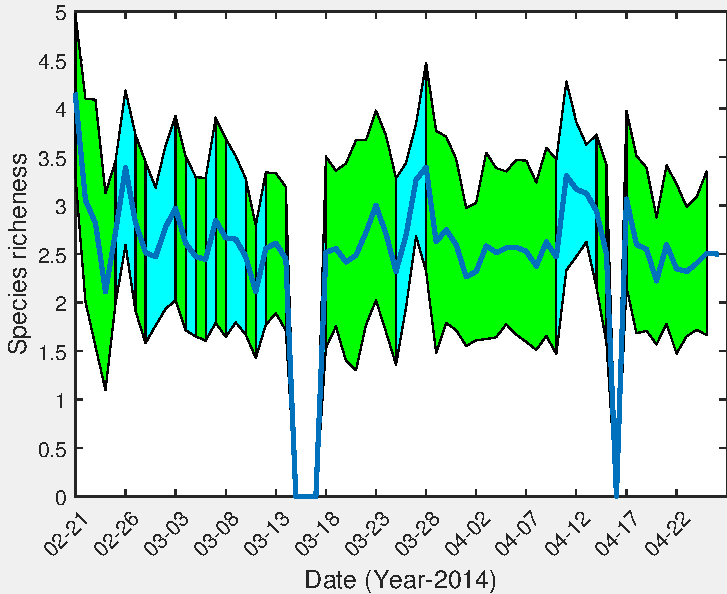
\includegraphics[width=\textwidth]{image/Ch7/richness1075.pdf}
                \caption{\textit{Kiyomi dam}}
        \end{subfigure}
       ~
              \begin{subfigure}[b]{0.3\textwidth}
                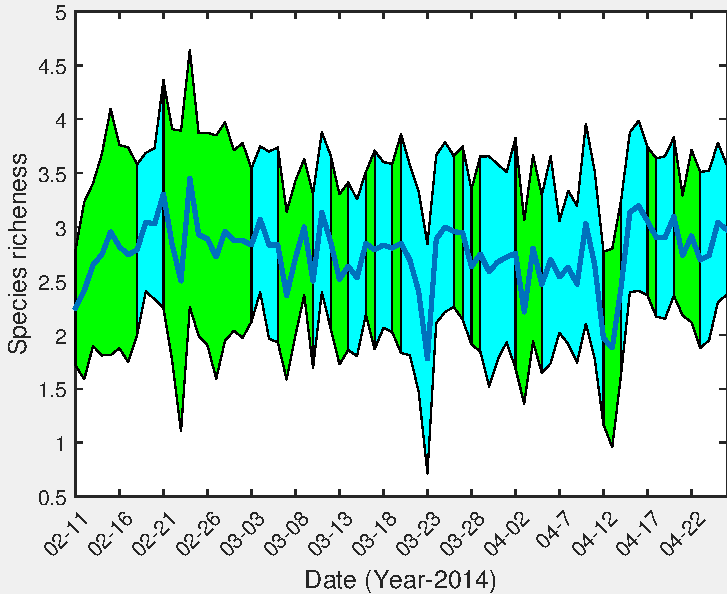
\includegraphics[width=\textwidth]{image/Ch7/richness1078.pdf}     
                \caption{\textit{Stony creek dam}}           
        \end{subfigure} 
        ~
              \begin{subfigure}[b]{0.3\textwidth}
                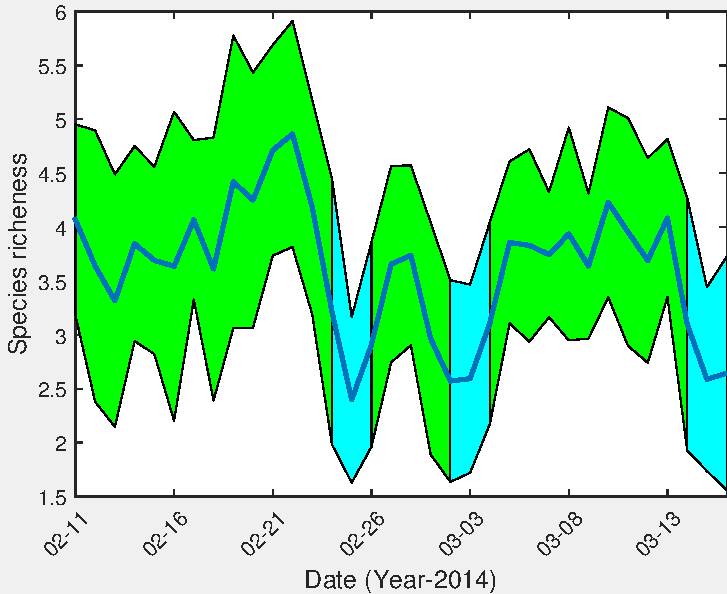
\includegraphics[width=\textwidth]{image/Ch7/richness1079.pdf}     
                \caption{\textit{BG creek dam}}           
        \end{subfigure}       
\caption[Frog species richness distribution of three selected sites]{Frog species richness distribution of three selected sites. Here green bar represents the species variation, blue bar means there is no frog calls, zero value denotes the data loss of those particular days.}
        \label{fig:frogRichness}
\end{figure}

\begin{figure}[htb!]
	\begin{centering}
	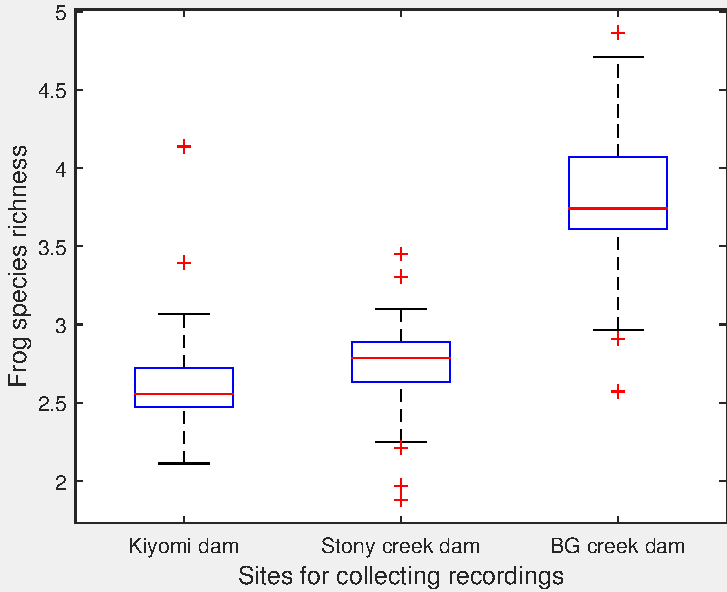
\includegraphics[width=0.5\textwidth]{image/Ch7/richnessSite.pdf}
	\caption{Averaged frog species richness of different sites.}
	\label{fig:richnessSite}
	\end{centering}
\end{figure}



\subsection{Comparison with MIML}
In this chapter, ML learning is used to classify frog calls without syllable segmentation. Compared with the MIML learning (Table~\ref{tab:accuracy} in chapter \ref{cha:cha6MIML}), the ML classification has a better classification performance. Although extracting global features for the ML classification will lose some detailed information, most frog vocalisations can still be successfully described when using cepstral features.
Compared with other features, global cepstral features are often calculated from each windowed signal. Then, the statistical results, such as mean and standard deviation, of all the windowed signals are calculated, this process will compress the information in the time domain but keep the information of the frequency domain. Since most frogs tend to continuously make calls, the compression of the time domain information will not greatly affect the discriminability of the ceptral features. In contrast, MIML classification needs to conduct the syllable segmentation before feature extraction. However, the use of AED often cannot accurately segment frog calls with low energies, which greatly affects the performance.








\section{Statistical analysis}
Multiple regression analysis is used to explore the relationship between frog calling activity/species richness with weather variables (mean temperature and rainfall)\footnote[5] {http://www.bom.gov.au/?ref=hdr}. Both frog calling activity and species richness are found to be highly correlated with mean temperature (F=5.18, P\textless0.05 for calling activity, and F=10.7, P\textless0.01 for species richness). To calculate the correlation between rainfall and frog calling activity/species richness, we first set the rainfall vaule as the dummy variable. Then, the correlation between frog calling activity/species richness and rainfall value is also studied with multiple regression analysis (F=4.63, P\textless0.05 for calling activity, and F=4.64, P\textless0.05 for species richness). The statistical analysis results indicate that frogs tend to make calls in the warm and humid environment, which is in accordance to previous studies \citep{akmentins2015patterns, canavero2008calling}.





\section{Summary and limitations}
Acoustic sensors are more widely used to monitor frog calling activity and species richness than the traditional field survey method. However, the use of acoustic sensors generates large volumes of audio data, which makes it necessary to develop automated methods. This paper proposes a novel method for detecting frog calling activity and species richness based on AED and ML learning. Specifically,
AED is the first step to calculate frog calling activity. Meanwhile, those 10-second recordings without frog calls are filtered out. For those recordings with frog calls, ML learning is further used for estimating frog species richness with multi-stage PWSCCs and LPCs. Finally, statistical analysis is utilised to reflect the relationship between frog calling activity/species richness with weather variables (mean temperature and rainfall). Experimental results show that our proposed method can accurately estimate frog calling activity/species richness and reflect their relationship with weather variables. Future work will focus on a wider frog call database, including a larger number of frog species, and frog calls collected over a longer period.


